

\documentclass [12 pt ]{article}
\usepackage{graphicx}%for including graphics file
\usepackage{color}
\usepackage[margin=1in]{geometry}
%TITLE PAGE
\title{\textbf{\huge{SOFTWARE LAB\\[0.5 cm]EEP 702}\\[1.5 cm] Assignment 10\\[0.5cm]Land-Water Discrimination using Java\\[0.5 cm]}}%for title page
\author{ {Harshit Kumar Gupta} \\Entry No: 2013EET2369\\[0.4 cm] \\[0.4cm] Computer Technology\\ Department Of Electrical Engineering\\[1cm]

\includegraphics[scale = 0.4]{IITD.png}
\\[0.5 cm] \textbf{Indian Institute of Technology Delhi}}
\date{April 8, 2014}
%MAIN CONTENT
\begin {document}
\maketitle
\newpage
\tableofcontents
\newpage 

%PROBLEM STATEMENT 
 \section{Problem Statement}
 Develop an Java program which can accomplish following tasks:   
\begin{enumerate}

\item There is a mass of land containing some finites number of water bodies. Let the piece of land be represented by a 2-D matrix, whose each cell
represents a unit area. Value '0' of a cell denotes that it comes under land area and '1' denotes that it comes under water body.
If the cells connected by a 4-point connectivity forms a single water body, find the total number of water bodies.


\item If the cells connected by a 8-point connectivity forms a single water body, find the total number of water bodies.


\item Label the water bodies so that if user specifies a cell (m,n), the program must tell whether it
comes under a water body.


\end{enumerate}
    
 \newpage
 
%ABSTRACT
\section {Abstract}
The problem seems to have been designed to provide hand on experience with the concepts of Java. Java is the most used OOP language and was used to
solve the given problem






\newpage
 %Specifications and Assumptions
 \section{Specification And Assumption}
 \subsection{Specification}
 The specifications of the variables and functions in the program are described below:
  \begin{enumerate}
   
  \item A matrix simulates a map of pixels.
  \item Each pixel has value either 0 or 1.
  \item 1 represents water in a map and 0 represents land.
  \item Five point thory defines waterbody in first case and nine point theory defines it in another. Theory is given above in abstract.
  \item One point immediately left or right or up or down to a waterbody comes in its domain and is also a part of it.
  \item A map dimensions are programmable and can have any dimensional value.

  

 \end{enumerate}
 \subsection{ Assumptions }
 \begin{enumerate}
 \item There is finite dimansional values of map.
 \item 0 marked as land are used as separator of waterbodies.
 \item user input is read from file
 \end{enumerate}

 \newpage
 \subsection{ Execution Method }
 \begin{enumerate}
 \item write the size of matrix as input in file.
 \item then write the input matrix on the file 
 \item 
 \end{enumerate}

 \newpage
 \section{Flow Chart}
 The basic algorithm that is implemented is shown through the flow chart given below.

\begin{center}
\vspace{1cm}
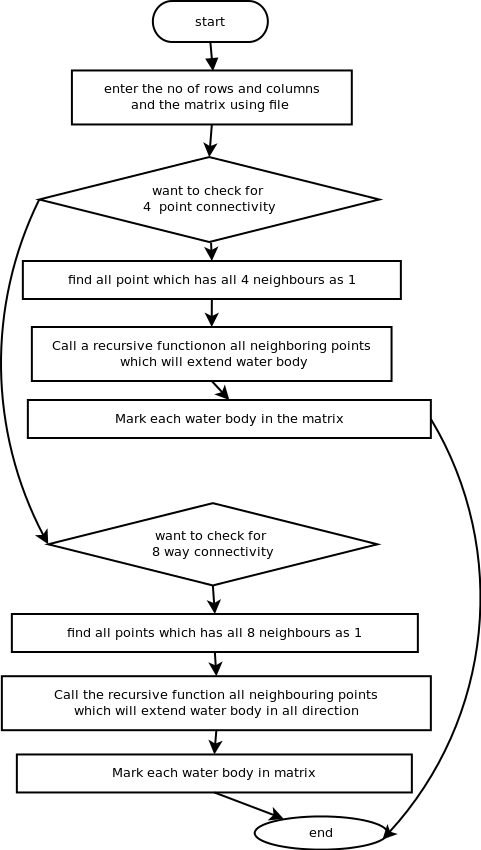
\includegraphics[height=18cm, width=15cm]{flowchart.png}

FIGURE 1: Flow Chart 
\end{center}-
\newpage
 
\section{Logic Implementation}
 The logic for Weather Forecasting is discussed below:
 
\begin{enumerate}
\item Initialy a random matrix is generated using the libray of python. The values of no of rows and columns are asked from the user.
\item A test is carried out on each point or each value in the matrix, to check whether that point is following adjacency criterion for 5 points or not.
\item If a point satisfies the criterion, it becomes the center of the waterbody. Now we have to expand our test points to all directions to see
whether this waterbody expands or not. 
\item If adjacent point is 1, it is part of waterbody, otherwise a 0 separates the waterbody from the land.
\item Control moves to next point and repeats point 2,3,4 on this point as well and so on till last point.
\item Point no 2,3,4,5, and 6 are gone through to discriminate land and water in case a waterbody's center follows 9 point adjacency.

  \end{enumerate}
 
 \newpage
 %Specifications and Assumptions



 
  \section{Result And Conclusion}
The conclusions drawn from the above programs are given below:

\begin{enumerate}
 \item Both programs worked for all possible combinations .
 \item Points that are 1 and are part of waterbody are marked as ####. 
 \item Points that are 1 and are not part of waterbody remains unmarked. 
 
 
\end{enumerate}
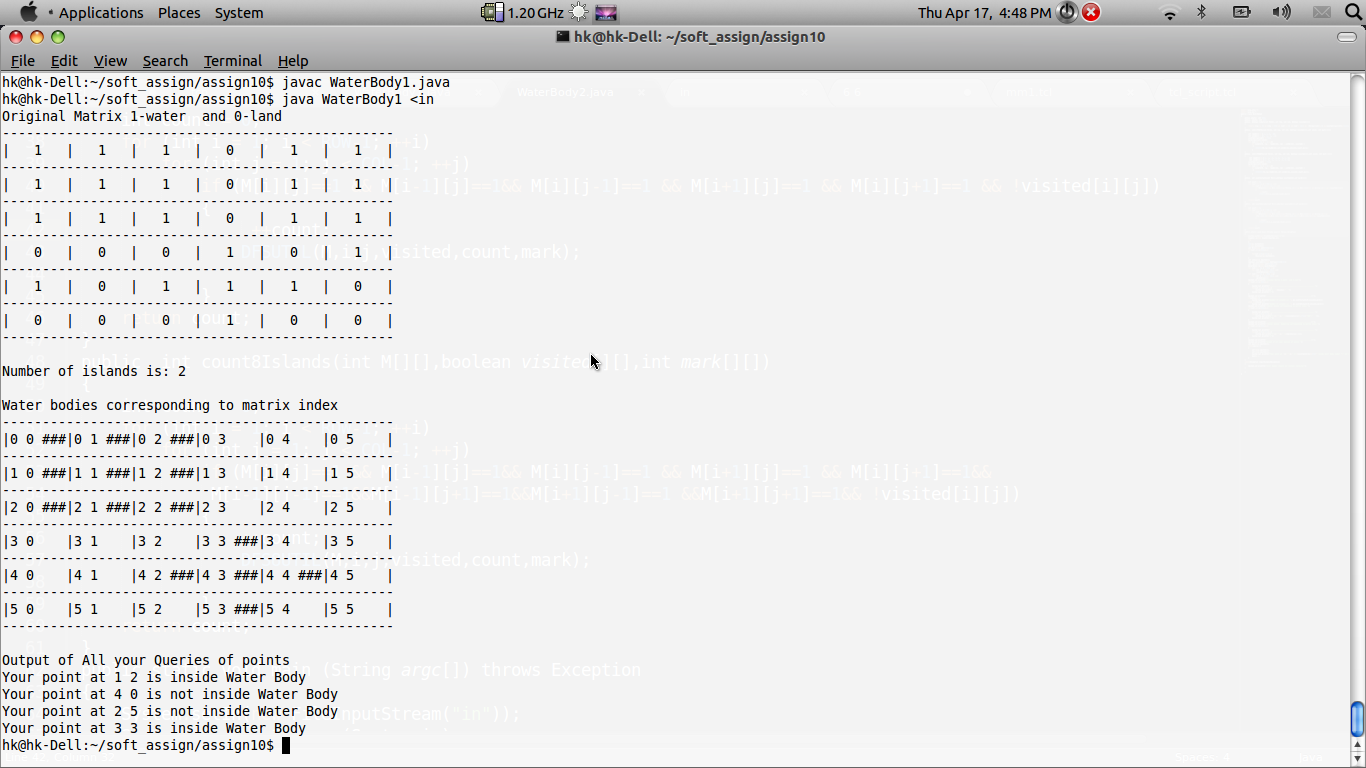
\includegraphics[height=18cm, width=15cm]{as.png}
 \end {document}